\section{Komponentenschnittstellen}
\textcolor{blue}{\textit{Hier sollen die Schnittstellen der in Abschnitt 1 eingeführten Komponenten definiert werden. Des Weiteren sollen hier Nachrichten, die eventuell  über die Schnittstellen verschickt werden, definiert werden. Nachrichten sind Klassen, die beispielsweise als Parameter der in den Schnittstellen deklarierten Operationen verwendet werden.
}}

\begin{figure}[H]
\centering
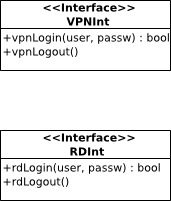
\includegraphics[width=0.3\textwidth]{img/Komponentenschnittstellen.png}
\caption{\textcolor{blue}{Durch eigenes Klassendiagramm ersetzen}}
\label{Komponentenschnittstellen}
\end{figure}
